\section{Lignes}
		
	Il existe plusieurs types de lignes:
	\begin{itemize}
		\item unifilaire
		\item bifilaire
		\item coaxiale
		\item fibre optique
		\item à ruban
		\item \dots
	\end{itemize}
		
		Elles dépendes de leur géométrie, des matériaux et des conditions, \dots
		
	\subsection{Modélisation d'une ligne}
	
		Une ligne est représentée comme  une résistance $R'$ ($\Omega/m$), une conductance $G'$, une inductance $L'$ et une capacité $C'$. Le morceau représenté si dessous se répète tous le long de la ligne.
		
		\begin{figure}[H]
			\centering
			\includegraphics[width=0.6\textwidth]{img/ModélisationLigne.png}
		\end{figure}		
		
		\begin{itemize}
			\item \textbf{$R'$} : Résistance du matériau (cuivre) qui transmet le signal $\rightarrow$ atténuation.
			\item \textbf{$L'$} : Inductance champ magnétique produit par un fil et qui impacte l'autre.
			\item \textbf{$C'$} : Effet de capacité entre les 2 fils.
			\item \textbf{$G'$} : Conductance, très grande résistance entre les 2 fils (air ou isolant) mais courant peut tout de même parfois passer légèrement à travers.
		\end{itemize}
		
		Ces paramètres varient suivant le type de ligne, la fréquence ou le matériel utilisé.
		
		L'équations des télégraphistes nous donnent la relation suivante :
		\begin{equation}
			\cfrac{\delta^2v}{\delta z^2} = LC\cfrac{\delta^2 v}{\delta t^2} + (RC + LG)\cfrac{\delta v}{\delta t} + RGv
		\end{equation}
		
		Si les pertes sont négligeables \textit{(R = G = 0)} :
		\begin{equation}
			\cfrac{\delta^2 v}{\delta z^2} = LC\cfrac{\delta^2 v}{\delta t^2}
		\end{equation}
		
		Elle fait le lien entre la variation de la tension en fonction de la position et un variation de la tension en fonction du temps.
		
		
	\subsection{Effet pelliculaire}
		Effet électromagnétique qui repousse les lignes de courant  vers la surface du conducteur. Les électrons vont s'amasser sur les bords.
		Diminue la surface de la ligne qui est effectivement parcourue par du courant et donc augmente la resistance de celui-ci comme $\sqrt{f}$, il est causé par la création d'un champ magnétique.
		
		\begin{align*}
			\nearrow \text{fréquence} \Rightarrow \nearrow \text{effet péliculaire} \Rightarrow \nearrow \text{résistance} \Rightarrow \nearrow \text{pertes}
		\end{align*}
			
	\subsection{Atténuation}
		Peut être calculé comme $10\log(P_{1}/P_{2})$, avec $P_1$ la puissance d'entrée et $P_2$ la puissance de sortie. Cette atténuation se calcule en dB(décibels).
		
		On sait que $P = \cfrac{V^2}{R}$, donc $\cfrac{P_1}{P_2} = \cfrac{v_{1}^{2}}{v_{2}^{2}}$
		
		\begin{equation}
			10\log(P_{1}/P_{2}) = 10\log(\cfrac{v_{1}^{2}}{v_{2}^{2}}) = 20\log(\cfrac{v_{1}}{v_{2}})
		\end{equation}
		
	\subsection{Dispersion}
		La \textbf{Dispersion} est une sorte de distorsion du signal et donc qui impacte l'information.
		
		Soit le nombre de pulsion $\omega = 2 \pi f$, le vecteur d'onde $\beta = \cfrac{2\pi}{\lambda}$, et $\lambda$ la longueur d'onde, on a la vitesse de phase (vitesse de propagation).
		\begin{equation}
			v_{ph} = \cfrac{\omega}{\beta}
		\end{equation}
		
		La dispersion d'un signal vient des différentes vitesses de déplacement des fréquences constituant une onde. L'onde a tendance à s'étaler sur le temps plus la ligne est longue.
		
	\subsection{Impédance caractéristique}
		Permet de connaitre le rapport de tension/courant utile dans beaucoup de systèmes pour savoir quelle tension on va récupérer en envoyant un certain courant. \textbf{Impédance caractéristique} désigne l'impédance en supposant que la ligne est infinie.
		
		La loi de Ohm caractérise une tension $v$ en fonction d'un résistance $r$ (ou $z$ pour résistances avec des nombres complexes) et d'un courant $i$.
		\begin{equation}
			v = ri\  \text{ou} \  v = zi
		\end{equation}
		
		$z$ est totalement réel pour une résistance pure et totalement imaginaire pour une inductance/capacité pure.
		
		Dans le cas d'une ligne infinie, l'impédance d'entrée est égal à l'impédance caractéristique de la ligne $Z_{in} = Z_c$\footnote{Voir slide 26 chap 2}.
		
	\subsection{Exposant de propagation}
		Il arrive que il y ait de la dispersion (déphasage) et de l'affaiblissement linéique (atténuation). Soit $\alpha$ l'atténuation et $\beta$ le déphasage, on peut calculer l'exposant de propagation $\gamma$:
		\begin{equation}
			\gamma = \sqrt{(R + j \omega L)(G + j \omega C)} = \alpha + j \beta
		\end{equation}
		
		Normalement, dans une ligne, $G$ est négligeable. Deux cas se présentent :
		
		\subsubsection{Cas 1}
			Dans le cas où, $\omega L << R$, correspond au cas où le fil a beaucoup de résistance.
			
			L'exposant de propagation en considérant $G$ et $\omega L$ nuls (car ils sont négligable au vu des hypothèses de ce cas) devient :
			
			\begin{figure}[H]
				\centering
				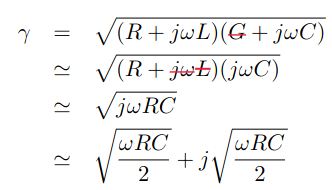
\includegraphics[width=0.4\textwidth]{img/1.png}
			\end{figure}	
			
			L'impédance caractéristique en considérant $G$ et $\omega L$ nul devient :
			
			\begin{figure}[H]
				\centering
				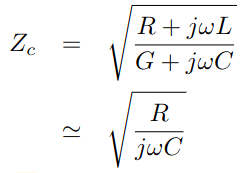
\includegraphics[width=0.3\textwidth]{img/2.png}
			\end{figure}	
				
		\subsubsection{Cas 2}
			Dans le cas où, $\omega L >> R$, correspond au cas où le fil a peu de résistance.
			C'est une bonne situation car il y a peu de distortion.
			
			L'exposant de propagation en considérant $G$ nul (car il est négligable) devient :
			
			\begin{figure}[H]
				\centering
				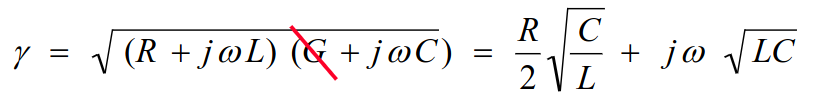
\includegraphics[width=0.6\textwidth]{img/3.png}
			\end{figure}	
			
			L'impédance caractéristique en annulant $G$ et $R$.
			
			\begin{figure}[H]
				\centering
				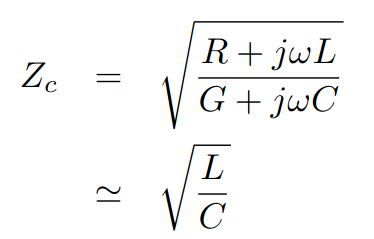
\includegraphics[width=0.2\textwidth]{img/4.png}
			\end{figure}	
			
			$\alpha$ est indépendant de $\omega$ et $\beta$ proportionnel à $\omega$. À cela s'ajoute $Z_c$ qui est réel et indépendant de $\omega$.
			
						
	\subsection{Pupinisation}
	
		Le cas des anciennes lignes téléphonique basse fréquences. Plus utilisé maintenant avec ADSL/VDSL.
		
		Pour le cas d'une ligne téléphonique $\omega L << R$, on va faire une pupinisation. C'est le fait d'insérer des inductances le long de la ligne pour augmenter artificiellement L. Avec ça, on a une réduction de l'atténuation le long de la ligne. On crée un filtre passe-bas.
		
		Mais cela n'est pas très bénéfique pour une certaine bande de fréquences car elle cause l'atténuation des fréquences supérieures. Vu qu'on a besoin de ces basses fréquences, on utilise plus cette technique \footnote{Voir graph Slides 34-35 chap 2}.
		
	\subsection{Lignes Bifilaire}
	
		Lignes constituée de fils parallèles séparés par un isolant, souvent rassemblé dans des quartes torsadées (quatre fils ensembles) ou encore dans une bottes de quartes (50 fils).
		
		On peut trouver de la Diaphonie (\textit{Bruit} / \textit{Crosstalk}). L'interférence d'un premier signal avec un autre (on peut par exemple entendre une autre conversation) qui passe dans un fil différent.
		
		Avantage :
		\begin{itemize}
			\item Faible coût
			\item Connexion facile
			\item Pré-installation dans les bâtiments
		\end{itemize}
		
		Déavantage :
		\begin{itemize}
			\item Faible atténuation aux basses fréquences
			\item Rayonnement important (problème de confidentialité, sensibilité aux interférences)
		\end{itemize}

\begin{figure}[H]
\centering
\begin{minipage}{.5\textwidth}
  \centering
  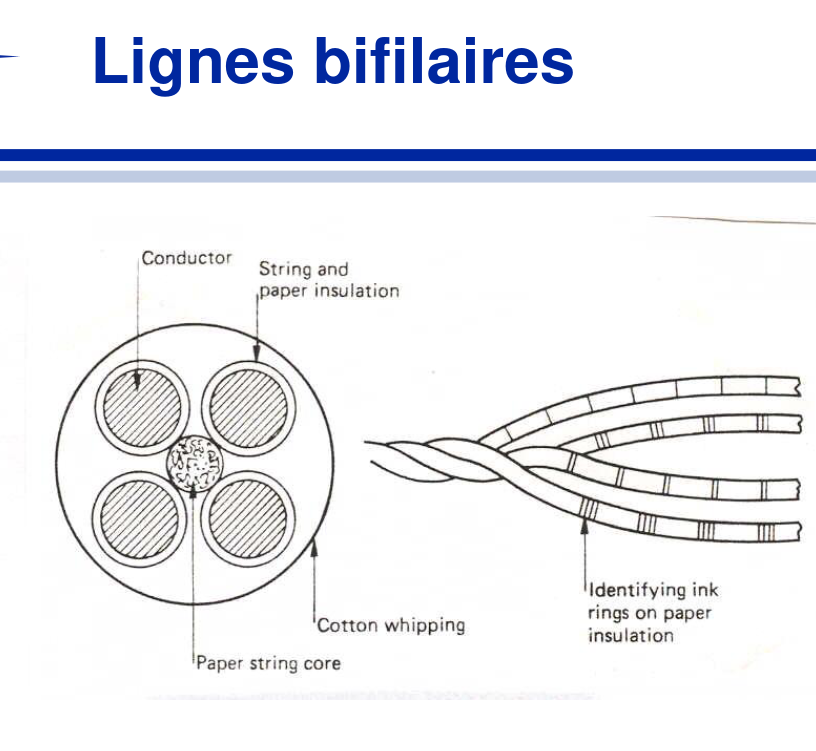
\includegraphics[width=.5\textwidth]{img/bifillaire.png}
\end{minipage}%
\begin{minipage}{.5\textwidth}
  \centering
  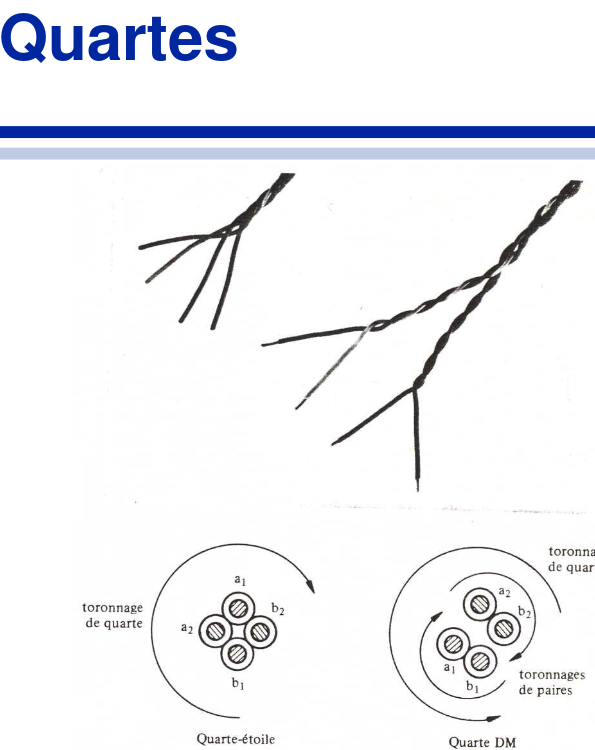
\includegraphics[width=.5\textwidth]{img/bifillaire2.png}
\end{minipage}
\begin{minipage}{.5\textwidth}
  \centering
  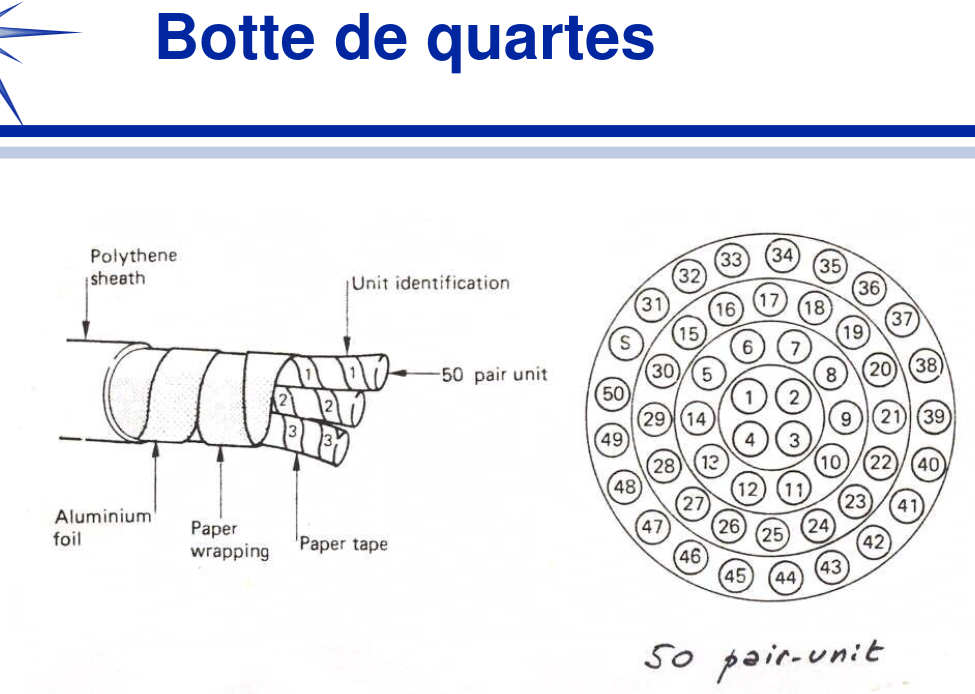
\includegraphics[width=.7\textwidth]{img/bifillaire3.png}
\end{minipage}

\end{figure}		
		
	\subsection{Cable coaxial}
		Câble composé d'une partie centrale (fil de cuivre) enveloppée d'un isolant, puis d'un blindage métallique tressée et enfin d'une gaine extérieure. Ce câble est utilisé pour la transmission de la télédistribution.
		
		Avantages :
		\begin{itemize}
			\item Large bande passante (\sim 500 MHz)
			\item Protection contre les interférences
			\item Technique éprouvée et répandue
			\item Facilité de réparation et de connexion
		\end{itemize}
		
		Désavantages :
		\begin{itemize}
			\item Fréquence limitée (\sim 500 MHz)
			\item Blindage jamais parfait
		\end{itemize}
		
		\begin{figure}[H]
\centering
\begin{minipage}{.5\textwidth}
  \centering
  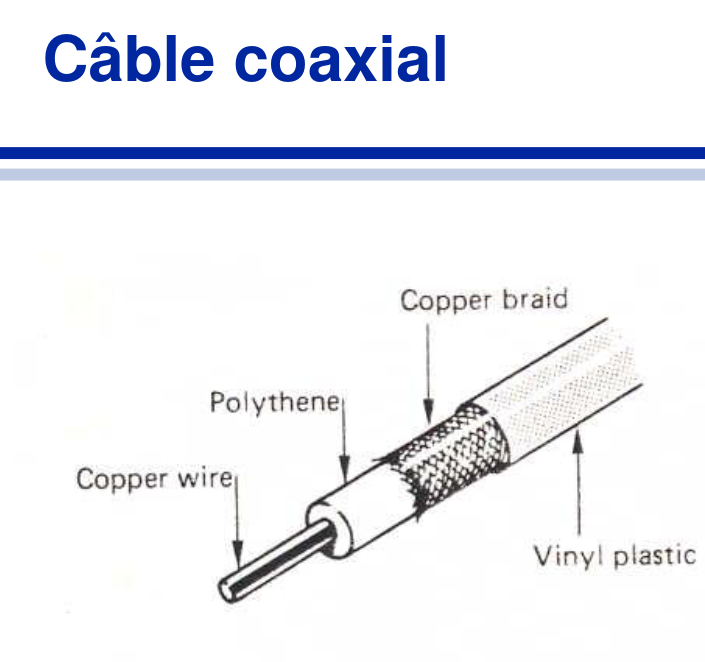
\includegraphics[width=.6\textwidth]{img/coaxial1.png}
\end{minipage}%
\begin{minipage}{.5\textwidth}
  \centering
  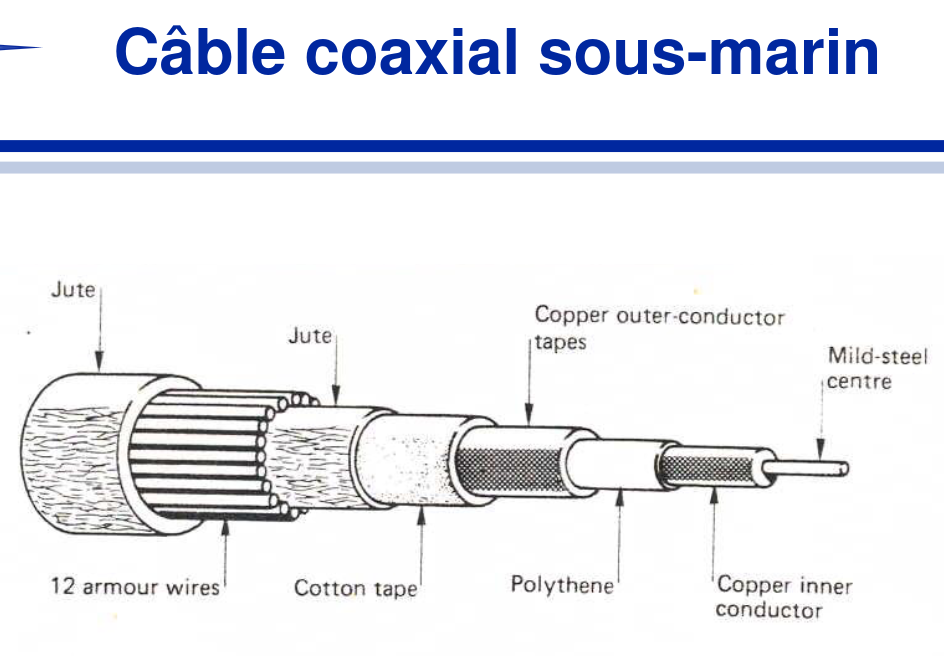
\includegraphics[width=.6\textwidth]{img/coaxial2.png}
\end{minipage}
\begin{minipage}{.5\textwidth}
  \centering
\end{minipage}

\end{figure}		

	\subsection{Fibre optique}
		C'est un conducteur de lumière en fil en verre ou plastique très fin qui transmet les données sous forme de lumière.
		
		Un \textbf{Mode} est un chemin emprunté par la lumiere par rapport à sa réflexion et réfraction dans la fibre optique.
		
		La \textbf{Dispertion intermodale} c'est un phénomène correspondant à l'existence de différentes vitesses possible pour la propagation des ondes. La distance parcourue par certains modes est différente de celle d'autre mode, il y a donc une dispersion du signal.
		
		Il y a plusieurs moyens d'envoyer un signal lumineux :
		\begin{itemize}
			\item Diode LED
			\item Diode Laser
			\item Diode Infrarouge
		\end{itemize}

		\textbf{Avantages :}
		\begin{itemize}
			\item Énorme bande passante
			\item Très faible attenuation
			\item Immunité à l'égard des rayonnement
			\item Isolation électrique
			\item Léger, fin, pas cher
		\end{itemize}
		
		\textbf{Désavantages :}
		\begin{itemize}
			\item Connexions difficiles
			\item Réparations difficiles
			\item Toujours en développement
		\end{itemize}
		
		\subsubsection{Manières de gérer les modes}
			\begin{enumerate}
				 \item \textbf{Fibre multimode à saut d'indice} : Les rayons réfléchissent plusieurs fois sur les parois avec un multitude d'angles différents. Le saut d'indice engendre des angles très fluctuants, il y a donc de la dispertion intermodale.
				 \begin{figure}[H]
				 	\centering
				 	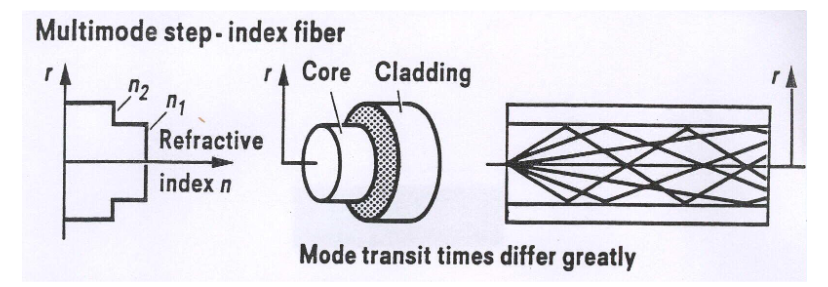
\includegraphics[width=\textwidth]{img/multimode.png}
				 \end{figure}
				 
				 \item \textbf{Fibre multimode à gradient d'indice} : On fait varier l'indice de réfraction plus l'on s'apporchera des parois afin que les différents faisceaux lumineux convergent vers le centre de la fibre. La dispersion intermodale est réduite.
				 
				 \begin{figure}[H]
				 	\centering
				 	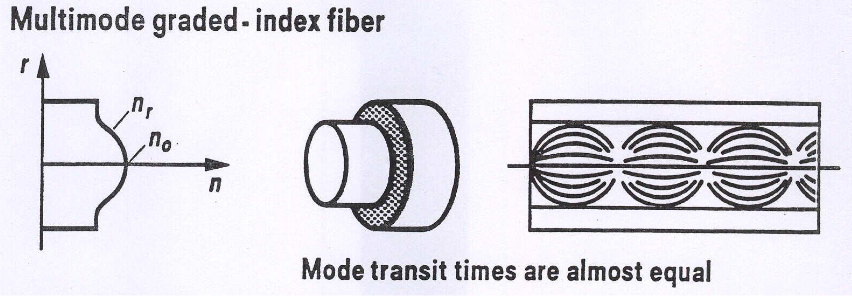
\includegraphics[width=\textwidth]{img/multimode2.png}
				 \end{figure}
				 
				 \item \textbf{Fibre Monomode} : un seul chemin au centre de la fibre. Une seule vitesse dans la fibre donc pas de dispertion intermodale.
				 
				 \begin{figure}[H]
				 	\centering
				 	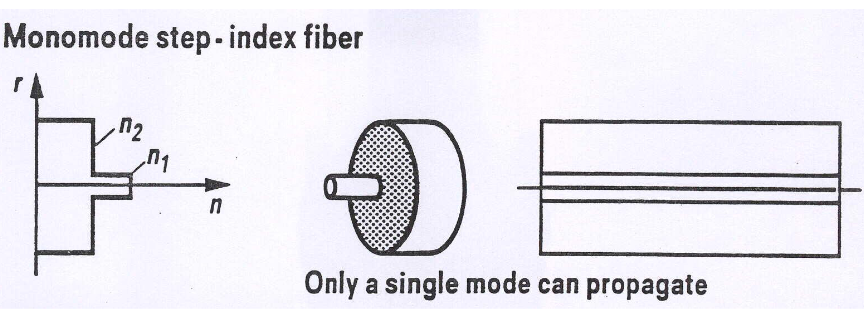
\includegraphics[width=\textwidth]{img/multimode3.png}
				 \end{figure}
			\end{enumerate}
			
			\subsubsection{Transmission dans une fibre optique}
				Un rayon rentre dans la fibre optique et est réfléchi à l'intérieur si celui-ci possède un angle adéquat qui est donc dans la range du cône d'appartenance et va parcourir la fibre optique en zigzag.
				